\section{Implémentation du modèle}

\begin{frame}

    \frametitle{Implémentation}
    \framesubtitle{Plan}
    \textbf{Implémentation}
    \begin{itemize}
        \item <2-> Choix d'implémentation
        \item <3-> Construction de la matrice d'adjacence
        \item <4-> Implémentation des algorithmes
    \end{itemize}
\end{frame}


\begin{frame}
    \frametitle{Implémentation}
    \framesubtitle{Choix}
    Deux algorithmes connus de recherche du plus court chemin :
    \begin{itemize}
        \item <2-> Dijkstra
        \item <3-> $\text{A}^{*}$
    \end{itemize}
    \bigskip
    Ceux-ci sont basés sur l'étude d'un \textbf{graphe associé} au problème
\end{frame}


\begin{frame}
    \frametitle{Implémentation}
    \framesubtitle{Graphe associé}
    On définit le graphe associé à une carte $M$ par :
    \bigskip
    \begin{align*}
        \onslide<2-> G_M =         & (S, A)                                                           \\
        \onslide<3-> \text{ avec } & S = \{u \in M \colon u \text{ est une position valide}\},        \\
        \onslide<4->               & A = \{(u,\ v)\in S \colon u \text{ et } v \text{ sont voisins}\}
    \end{align*}

\end{frame}


\begin{frame}
    \frametitle{Implémentation}
    \framesubtitle{Matrice d'adjacence}

    Dans le programme, le graphe $G_M$ est représenté par une matrice d'adjacence $A_G$ définie par :

    \begin{align*}
        \onslide<2-> S & = \{0, 1, \dots, n \times p - 1 \}                                                                                        \\
        \bigskip
        \onslide<3->   & \forall (i,j)\in \llbracket 0, n-1\rrbracket \times \llbracket 0, p-1\rrbracket,\space A_{G_{i,j}} = \mathbb{1}_{A} (i,j)
    \end{align*}
\end{frame}


\begin{frame}
    \frametitle{Implémentation}
    \framesubtitle{Algorithme}
    Algorithme utilisé : \bigskip
    \textbf{A*}
    \begin{itemize}
        \item <2-> Approxime le plus court chemin à l'aide d'une heuristique
        \item <3-> Explore le graphe en estimant la pertinence de chaque nœud pour se rendre à l'objectif
    \end{itemize}
\end{frame}


\begin{frame}
    \frametitle{Implémentation}
    \framesubtitle{Heuristique}
    Une heuristique est une application de la forme :
    \onslide<2->{
        \begin{empheq}[left=h \colon \empheqlbrace]{align*}
            \mathbb{R}^2 \times \mathbb{R}^2 \times M_{n,p}(\mathbb{N}) \to& \mathbb{R}\\
            (pos, pos_{but}, M) \mapsto& h(pos, pos_{but}, M)
        \end{empheq}
    }
    \onslide<3->{
        Exemple : la norme euclidienne
        \begin{empheq}[left=h \colon \empheqlbrace]{align*}
            \mathbb{R}^2 \times \mathbb{R}^2 \times M_{n,p}(\mathbb{N}) \to& \mathbb{R}\\
            ((x,y), (x', y'), M) \mapsto& \sqrt{(x'-x)^2 + (y-y')^2}
        \end{empheq}
    }
\end{frame}


\begin{frame}
    \frametitle{Implémentation}
    \framesubtitle{Cadre des tests}
    \textbf{Cadre} : quai de métro à l'arrivée d'un train (partie supérieure) et disposant de plusieurs accès (partie inférieure) \\[.3cm]
    \onslide<2-> Une case correspond à \num{1}\si{\metre \squared}, avec une limite de 6 \si{personnes \per \metre \squared}
    \onslide<3->{
        \begin{figure}
            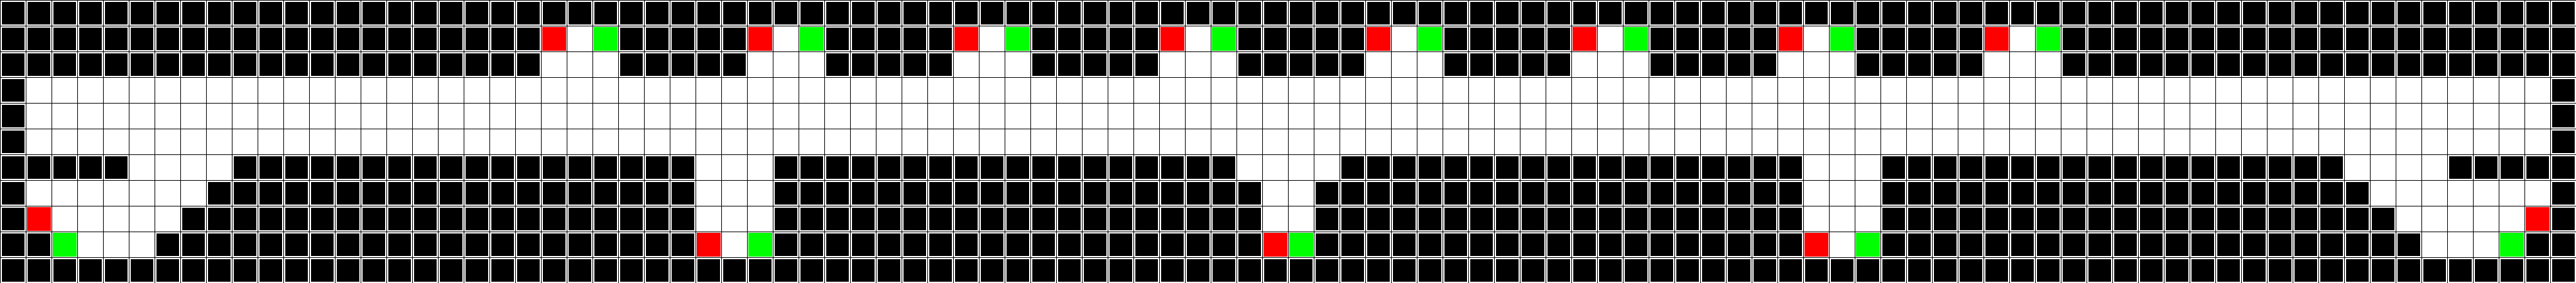
\includegraphics[width=1\textwidth]{figures/Fig05}
        \end{figure}
        \fcolorbox{black}{black}{\rule{0pt}{6pt}\rule{6pt}{0pt}}\quad Mur (case infranchissable) \\
        \fcolorbox{black}{white}{\rule{0pt}{6pt}\rule{6pt}{0pt}}\quad Quai (case franchissable) \\
        \fcolorbox{black}{green}{\rule{0pt}{6pt}\rule{6pt}{0pt}}\quad Sortie \\
        \fcolorbox{black}{red}{\rule{0pt}{6pt}\rule{6pt}{0pt}}\quad Entrée \\
    }
\end{frame}


\begin{frame}
    \frametitle{Implémentation}
    \framesubtitle{Test norme euclidienne}
    \textbf{Résultats du programme :} \\
    \onslide<2-> {Pour de petites populations initiales la simulation se \textbf{termine correctement} \\[.1cm]}
    \onslide<3->{Pour une population initiale de \textbf{600 agents}, la simulation n'aboutit pas à une évacuation complète :}
    \begin{figure}
        \only<3->{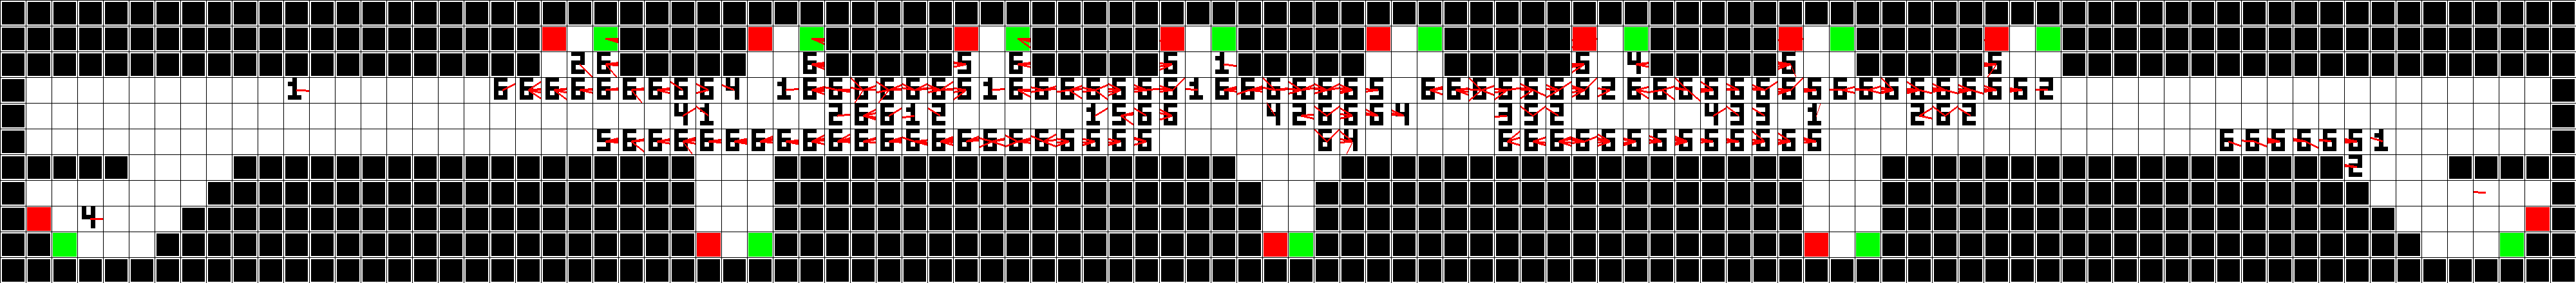
\includegraphics[width=1\textwidth]{figures/Fig03}\\[.5cm]}
        \begin{columns}
            \only<3->{
                \begin{column}{0.475\textwidth}
                    La simulation est \textbf{figée} de manière non réaliste : \\[.1cm]
                    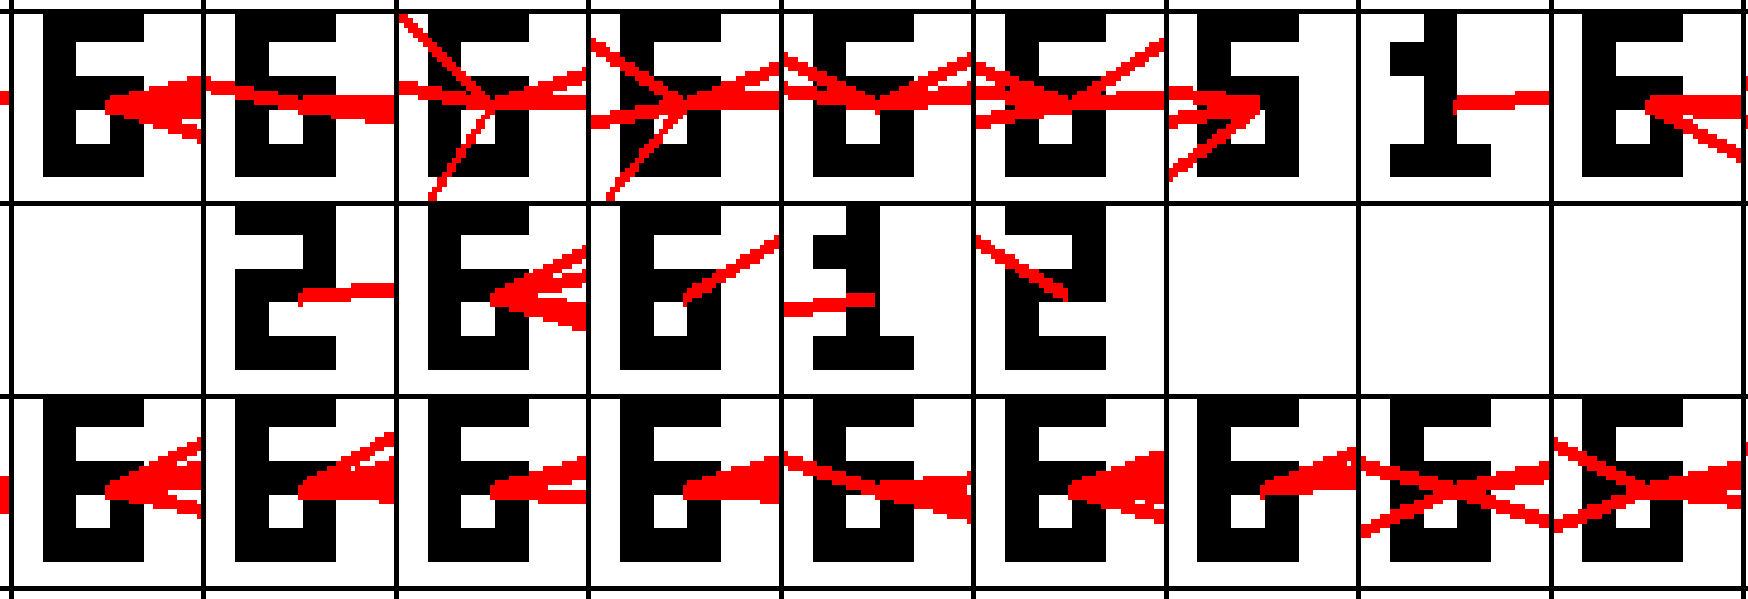
\includegraphics[width=.9\textwidth, left]{figures/Fig04}
                \end{column}
            }
            \only<4->{

                \begin{column}{.5\textwidth}
                    Cette heuristique n'est correcte que dans le cas d'un graphe constant. Or notre graphe varie en fonction des agents à proximité.
                \end{column}
            }
        \end{columns}
    \end{figure}
\end{frame}


\begin{frame}
    \frametitle{Implémentation}
    \framesubtitle{Une nouvelle heuristique}
    On cherche alors à modifier notre heuristique pour
    \begin{itemize}
        \item <2-> la rendre plus réaliste
        \item <3-> prendre en compte les agents à proximité
    \end{itemize}

\end{frame}


\begin{frame}[fragile]
    \frametitle{Implémentation}
    \framesubtitle{Proposition d'une heuristique}
    On ajoute pour cela un paramètre \textit{REPULSION} à la simulation :
    \begin{onslide}<2->
        \begin{code}
            \begin{minted}[linenos]{c}
int h(location pos, location goal, map *m) {
    int f = 1;
    for (int i=0; i<REPULSION; i++) {
        f*=m->level[pos.y][pos.x];
    }
    return f
           + (goal.x - pos.x) * (goal.x - pos.x)
           + (goal.y - pos.y) * (goal.y - pos.y);
}
    \end{minted}
        \end{code}
        Après avoir testé différentes valeurs, on a estimé que la valeur \textbf{4} renvoyait un résultat convenable.
    \end{onslide}


\end{frame}


\begin{frame}
    \frametitle{Implémentation}
    \framesubtitle{Test de cette nouvelle heuristique}
    \textbf{Résultats du programme :} \\
    \onslide<2->{Pour une population initiale de \textbf{600 agents}, la simulation ne rencontre plus de blocage.\\[.2cm]}
    \onslide<3->{Le nouveau blocage est rencontré pour des populations initiales \textbf{supérieures à 1000 agents.}}
    \begin{figure}
        \onslide<4->{
            Le mouvement est maintenant limité par l'agencement même du lieu :\\[.1cm]}
        \only<4>{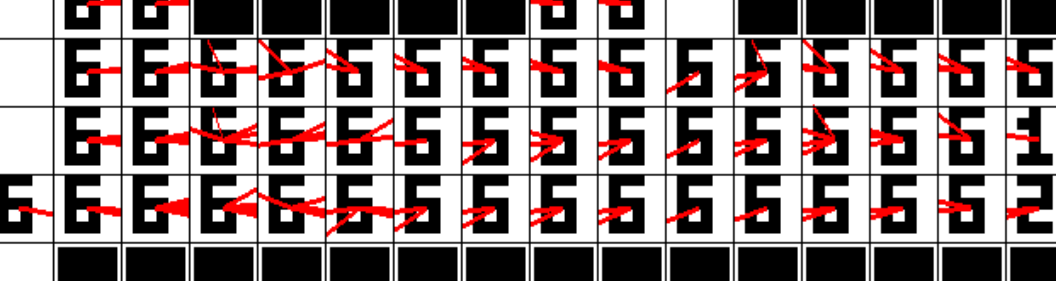
\includegraphics[scale=0.3]{figures/Fig06}}
    \end{figure}
\end{frame}


\begin{frame}
    \frametitle{Implémentation}
    \framesubtitle{Déplacements plus réaliste}
    On cherche maintenant à obtenir un déplacement plus réaliste en introduisant des limites de densité : \\
    \begin{itemize}
        \item <2-> Densité acceptable : 3 p/m²
        \item <3-> Densité maximale : 6 p/m²
    \end{itemize}
    \bigskip
    \onslide<4->{Si la case visée contient N agents, le déplacement est possible si :}
    \begin{itemize}
        \item <5-> $N<3$
        \item <6-> $2 <N< 6$ et l'agent subit des pressions extérieures de la part d'au moins deux agents
    \end{itemize}
\end{frame}


\begin{frame}
    \frametitle{Implémentation}
    \framesubtitle{Résultats de cette nouvelle fonction}
    La nouvelle fonction permet un déplacement plus réaliste des agents qui s'éparpillent dans l'espace après être entrés dans la pièce. \\[.1cm]
    \begin{figure}
        \centering
        \begin{subfigure}{.5\textwidth}
            \centering
            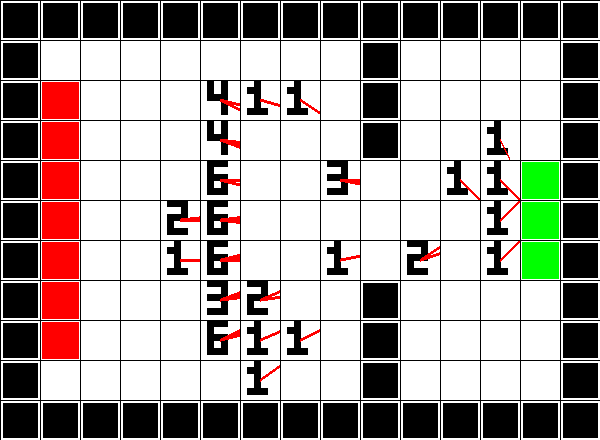
\includegraphics[scale=0.2]{figures/Fig10}\caption{Ancienne fonction}
            \label{fig:sub1}
        \end{subfigure}%
        \begin{subfigure}{.5\textwidth}
            \centering
            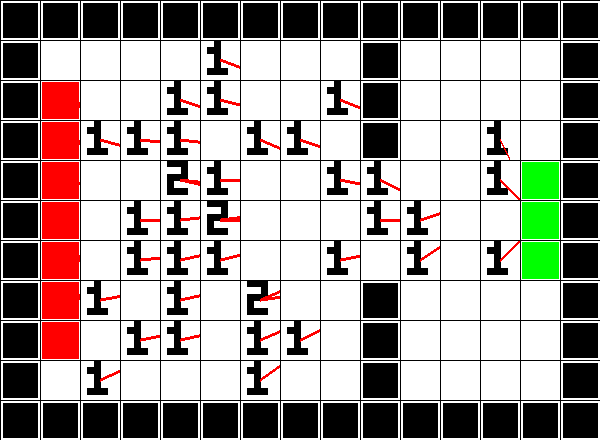
\includegraphics[scale=0.2]{figures/Fig11}
            \caption{Nouvelle fonction}
            \label{fig:sub2}
        \end{subfigure}
        \label{fig:test}
    \end{figure}
    \tiny{
        \fcolorbox{black}{green}{\rule{0pt}{6pt}\rule{6pt}{0pt}}\quad Sortie \
        \fcolorbox{black}{black}{\rule{0pt}{6pt}\rule{6pt}{0pt}}\quad Mur (case infranchissable)\\
        \fcolorbox{black}{red}{\rule{0pt}{6pt}\rule{6pt}{0pt}}\quad Entrée
        \fcolorbox{black}{white}{\rule{0pt}{6pt}\rule{6pt}{0pt}}\quad Air (case franchissable)
    }
\end{frame}